\documentclass[11pt]{article}

% ------------------------------------------------------------------
% Plain-LaTeX version of the CS224N final-report layout so it compiles anywhere.
% To use the official template, copy everything between \begin{document}
% and \end{document} (and refs.bib) into the template's main.tex.
% ------------------------------------------------------------------
\usepackage[margin=1in]{geometry}
\usepackage[T1]{fontenc}
\usepackage{times}
\usepackage{microtype}
\usepackage{amsmath,amssymb}
\usepackage{graphicx}
\usepackage{booktabs}
\usepackage{multirow}
\usepackage{array}
\usepackage[numbers,sort&compress]{natbib}
\usepackage[hidelinks]{hyperref}
\usepackage{caption}
\captionsetup{font=small,labelfont=bf}
\setlength{\parskip}{3pt}
\renewcommand{\arraystretch}{1.05}

\newcommand{\dpen}{\textit{dp}}
\newcommand{\spen}{\textit{sp}}
\newcommand{\score}{\textsc{Score}}

\title{\vspace{-1.2em}\textbf{Pixels to Power Pellets: Reward Shaping, Input Modality and Architecture\\ in Pixel-Based PPO for Ms.\ Pac-Man}}
\author{
  Le Minh Khoi \\ \texttt{SE192396} \and
  Pham Quang Huy \\ \texttt{SE184775} \and
  Ngo Quang Huy \\ \texttt{SE190631} 
}
\date{}

\begin{document}
\maketitle

\section*{Key Information to Include}
\vspace{-0.5em}
\begin{itemize}\setlength{\itemsep}{0pt}
  \item \textbf{Team contributions:} [Member 1: PPO/DQN library, environment wrappers, reward shaping, penalty experiments.  Member 2: LSTM and ViT networks, RGB-from-gray conversion, evaluation, analysis and writing.] \emph{(Replace with the real split, 1--2 sentences per person.)}
  \item \textbf{Project type:} Reinforcement Learning.
  \item \textbf{Mentor:} NamLG
  \item \textbf{External collaborators:} None. \item \textbf{Shared project:} \url{https://github.com/Khoile5464/rel_ms_pacman}
  \item \textbf{Code:} \texttt{pacman\_rl} (PPO, DQN, vectorised environments, networks) and the notebooks that call it were written by us; the emulator and environment come from Gymnasium/ALE (see \S\ref{sec:approach}).
\end{itemize}

\begin{abstract}
Reinforcement-learning agents that play Atari from raw pixels are a standard testbed for deep policy-gradient methods, but a plain Proximal Policy Optimization (PPO) agent on Ms.\ Pac-Man quickly stalls at roughly 700 points, about 2.5$\times$ a random policy. We try to find out why and what moves it past that plateau. We implement PPO from scratch in PyTorch and run a chain of hypothesis-driven experiments: (H1) the agent idles because dying is cheap and waiting is free, so we add a death penalty (\dpen) and a per-step penalty (\spen); (H2) grayscale frames erase the colour of frightened ghosts, so we try RGB input and a gray-to-RGB weight-transfer scheme; (H3) a single frame lacks memory, so we compare a CNN with a CNN+LSTM and a small Vision Transformer (ViT). Over 23 saved training runs of 1--24 M agent steps (about 84 M steps in total), we find that (i) RGB input gives no measurable gain at 1--3 M steps; (ii) a large death penalty from the start hurts (499 vs.\ 651 points, two seeds); (iii) long, low-learning-rate fine-tuning with a small step penalty lifts the ViT to a training score of 1125 (median 975; best game 4720), driven by roughly doubling ghost captures per game; (iv) penalties that are too large make the agent collapse, and the value-loss scale gives an early warning of this. Our evaluation also shows 100--200 points of run-to-run noise on the same model, so many small differences cannot be interpreted. All figures are regenerated from the saved logs by a script in the project repository.
\end{abstract}

\section{Introduction}
\label{sec:intro}
Deep reinforcement learning (RL) from pixels, introduced for Atari by \citet{mnih2015dqn}, remains a central benchmark for learning from high-dimensional observations. Policy-gradient methods such as PPO \citep{schulman2017ppo} are popular because they are simple and robust, yet their behaviour in a specific game depends strongly on details that papers rarely foreground: reward scaling, how episodes are terminated, and how input frames are encoded \citep{engstrom2020implementation,huang2022ppo37,henderson2018matters}.

Ms.\ Pac-Man is a good case study. The reward is sparse in the sense that matters: ordinary dots give 10 points, but the large rewards (ghosts worth 200--1600 points) require a \emph{sequence} of decisions: eat a power pellet, notice that the ghosts have turned blue, chase them before the effect ends. Ghost movement is also stochastic, so there is no fixed route to memorise. When we trained a standard CNN-based PPO agent we saw the following: the score jumped within the first $\sim$25\,k steps, then stayed near 700 even when training was extended from 1 M to 2 M steps (random play scores 200--280). Watching the agent suggested it either stood still or repeated a fixed pattern, and that after eating a power pellet it did not hunt ghosts.

This report documents the diagnosis. We treat each suspected cause as a hypothesis and design the cheapest experiment that could confirm or reject it: reward shaping for idling (H1), RGB input for the lost ghost colour (H2), and recurrent or attention-based encoders for missing memory (H3). The contribution is \emph{not} a new algorithm, but (1) an end-to-end from-scratch PPO implementation with LSTM and ViT policies and a weight-transfer scheme from gray to RGB; (2) a controlled comparison of penalty schedules, input modality and architecture, with their negative results; (3) a quantified failure mode, penalty-induced collapse, together with a cheap diagnostic (the value loss); and (4) an honest look at evaluation noise, which affects how much of the RL literature's small gaps can be believed. Our best agent (a ViT fine-tuned over 13 M steps) reaches a mean training score of 1125, roughly four times random but far below human-level play.

\section{Related Work}
\label{sec:related}
\paragraph{Deep RL on Atari.} DQN \citep{mnih2013playing,mnih2015dqn} established learning from stacked 84$\times$84 gray frames with reward clipping, and Rainbow \citep{hessel2018rainbow} combined later improvements. The Arcade Learning Environment \citep{bellemare2013ale} and its evaluation protocol recommendations, including sticky actions \citep{machado2018revisiting}, define the benchmark. Actor-critic methods \citep{mnih2016a3c} and PPO \citep{schulman2017ppo} with generalised advantage estimation \citep{schulman2016gae} are the main on-policy alternatives. We use PPO because it parallelises easily on a single laptop GPU. Previous work on Ms.\ Pac-Man specifically decomposes the reward into per-object value functions \citep{vanseijen2017hra}; we instead keep a single scalar reward and ask which cheaper modifications help.

\paragraph{Implementation details and reproducibility.} \citet{engstrom2020implementation} and \citet{huang2022ppo37} show that code-level choices (reward normalisation, learning-rate annealing, value clipping) can matter as much as the algorithm, while \citet{henderson2018matters} and \citet{agarwal2021precipice} document how few seeds and noisy evaluation produce unreliable conclusions. These works motivate our decision to report evaluation noise explicitly and to flag every comparison that has only one seed.

\paragraph{Reward shaping.} Potential-based shaping preserves optimal policies \citep{ng1999shaping}, but a constant per-step cost or a death penalty is \emph{not} potential-based and can change the optimum. Reward misspecification is a known safety concern \citep{amodei2016concrete,skalse2022hacking}. Our collapse results (\S\ref{sec:analysis}) are a concrete small-scale instance.

\paragraph{Memory and attention in RL.} Recurrent Q-networks \citep{hausknecht2015drqn} use an LSTM \citep{hochreiter1997lstm} to handle partial observability. Transformers \citep{vaswani2017attention} and Vision Transformers \citep{dosovitskiy2021vit} are attractive encoders, but plain Transformers are known to be hard to train with RL objectives, which motivated stabilising variants \citep{parisotto2020gtrxl}. Because CS224N focuses on sequence models, we include both an LSTM and a ViT whose patch tokens are processed with self-attention, and compare them with the Nature-DQN CNN.

\section{Approach}
\label{sec:approach}
\paragraph{Vocabulary.} A \emph{step} is one agent decision (4 emulator frames). A \emph{life} ends when Pac-Man is caught; a \emph{game} is up to three lives. \score{} always means the real game score summed over a game (never the shaped reward). \emph{Training score} is the average \score{} of games finished during training (stochastic, drifting policy); \emph{evaluation score} is measured on separate games with a fixed seed set.

\subsection{Environment and reward}
We use \texttt{ALE/MsPacman-v5} from Gymnasium \citep{towers2023gymnasium} (code not ours): 9 discrete actions, frame-skip 4, no sticky actions. The observation is the last four frames, resized to 84$\times$84, stacked as $(4,84,84)$ for gray input or $(12,84,84)$ for RGB. During training, losing a life is reported as episode termination (``episodic life'') while the underlying game continues, so the value function sees shorter, well-defined episodes. For evaluation this wrapper is off and one full game is played (at most 4500 steps).

The learning reward is our own variant of reward compression (replacing clipping):
\begin{equation}
  \tilde r_t = \ln\!\bigl(1 + r_t/10\bigr) \;-\; \dpen\cdot \mathbb 1[\text{life lost at } t] \;-\; \spen,
  \label{eq:reward}
\end{equation}
where $r_t$ is the true game reward. A dot (10) gives $0.69$, a power pellet (50) gives $1.79$, and the four successive ghosts (200/400/800/1600) give $3.04/3.71/4.39/5.08$, so large events keep a larger, but not dominant, weight than clipping would allow. \dpen{} (death penalty) and \spen{} (per-step cost) implement H1.

\subsection{PPO}
We implemented PPO from scratch in PyTorch \citep{schulman2017ppo}: $N{=}32$ parallel environments $\times$ 512 steps per rollout (16\,384 samples per update), GAE with $\gamma{=}0.99$, $\lambda{=}0.95$ \citep{schulman2016gae}, and the clipped objective
\begin{equation}
  L = \mathbb E_t\!\Big[\min\!\big(\rho_t \hat A_t,\ \mathrm{clip}(\rho_t,1{-}\epsilon,1{+}\epsilon)\hat A_t\big)\Big] - c_1 \,\mathbb E_t\big[(V_\theta(s_t)-\hat R_t)^2\big] + c_2\, \mathbb E_t\big[\mathcal H(\pi_\theta(\cdot|s_t))\big],
\end{equation}
with $\rho_t=\pi_\theta/\pi_{\theta_{\text{old}}}$, $\epsilon{=}0.1$, $c_1{=}0.5$, $c_2{=}0.01$, 4 epochs, 4 minibatches, gradient-norm clip 0.5, Adam \citep{kingma2015adam} with linearly decayed learning rate (full list in Appendix~\ref{app:hparams}). Training used one RTX~3070~Ti laptop GPU.

\subsection{Policies}
All networks share an actor head (9 logits) and a critic head (scalar).
\begin{itemize}\setlength{\itemsep}{0pt}
  \item \textbf{CNN (baseline).} Nature-DQN trunk \citep{mnih2015dqn}: Conv(8$\times$8, s4)--Conv(4$\times$4, s2)--Conv(3$\times$3, s1)--FC-512.
  \item \textbf{CNN+LSTM.} Same trunk plus an LSTM (hidden 512). The hidden state is reset when a life is lost. Because the recurrent state must flow through a whole rollout, minibatches are formed by splitting environments (each keeps its 512-step sequence) rather than shuffling individual steps.
  \item \textbf{ViT.} A small Vision Transformer \citep{dosovitskiy2021vit}: 12$\times$12 patches ($7{\times}7{=}49$ tokens + a CLS token), width 128, depth 4, 4 heads, MLP ratio 2, pre-norm blocks \citep{xiong2020layernorm}, built on \texttt{torch.nn.TransformerEncoder}.
  \item \textbf{Gray-to-RGB weight transfer (ours).} To test colour without discarding what a gray agent has learned, we expand the first conv layer from 4 to 12 input channels by setting each frame's R, G, B weights to the gray weight $\times(0.299, 0.587, 0.114)$. This makes the RGB network's initial output approximately equal to the gray network's (the ITU-R 601 luminance mix), and all other layers are copied unchanged.
\end{itemize}

\subsection{Experimental protocol}
The study proceeded in five phases, each motivated by what the previous phase showed (\S\ref{sec:experiments}): \textbf{P0} baseline plateau (CNN gray, 2 M steps); \textbf{P1} penalty experiments (const-low, const-high, curriculum; 2 seeds, 1 M steps); \textbf{P2} gray vs.\ RGB and CNN vs.\ LSTM vs.\ ViT (1--3 M steps); \textbf{P3} long fine-tuning of LSTM and ViT (13 M steps in four stages) with a small step penalty and a lower learning rate; \textbf{P4} RGB networks initialised from gray with penalty ramps, including three step-penalty magnitudes.

\section{Experiments}
\label{sec:experiments}
\subsection{Data and task}
There is no fixed dataset: the agent generates its own experience from the emulator. Input is the 4-frame stack above; output is a distribution over 9 joystick actions. The goal is to maximise the game score over a three-life game.

\subsection{Evaluation method}
We report two quantities. (a) \textbf{Training score:} mean \score{} over the last 100--300 games of a run (the exact window is stated). It averages thousands of games, but it is measured with a stochastic policy that is still being updated, so it is biased low relative to a converged policy and only suitable for trends. (b) \textbf{Evaluation score:} 20 full games on seeds 1000--1019 with the policy \emph{sampled} (not greedy), reported as mean$\pm$std with the standard error $\approx\!\text{std}/\sqrt{20}$. We also track behavioural statistics from the game reward: ghosts eaten per game, power pellets per game, steps per game, and policy entropy (maximum $\ln 9 = 2.20$). Ghost and pellet counts come from exact reward matches (50 for a pellet, 200/400/800/1600 for a ghost); fruit worth 200 points from level~2 can occasionally be miscounted as a ghost. Random play scores 274 on average (5 games; other 5-game samples gave 198 and 282, so this baseline is itself noisy).

\subsection{Experimental details}
Unless stated, \dpen$=2.5$, \spen$=0$, learning rate $2.5\!\times\!10^{-4}$ (ViT: $10^{-4}$) decayed linearly to 0, 32 environments. Fine-tuning stages (P3) restart from the previous checkpoint with learning rate $10^{-4}$ or $5\!\times\!10^{-5}$ and \spen$=0.05$. Because each call to the trainer decays the learning rate to 0, long runs have a sawtooth schedule. Typical throughput was 240--260 agent steps/s (ViT); a 1 M-step run takes about an hour. Early in the project we found that a notebook cell had restarted from a fresh network at each call while appending logs to the same file, so what we thought was one run was in fact three concatenated runs. We fixed this and draw conclusions only from stages that we can verify.

\subsection{Results}
\paragraph{P0: the plateau.} The baseline CNN (gray, 16 environments, \dpen$=0$) reached 727 and 767 (mean of the last 100 games in two consecutive 2 M-step runs; the second started from the first). Entropy fell from 2.20 to $\approx\!1.2$ and the mean life length stayed at 205--220 steps for the whole run. Doubling the steps from 1 M to 2 M did not change the score, which ruled out ``just train longer'' at this learning rate as a quick fix.

\paragraph{P1: penalty schedules (H1).} Table~\ref{tab:penalty} compares a low constant penalty, a high constant penalty from step 0 (\dpen/\spen $=20/0.1$) and a curriculum that ramps from $2.5/0$ to $10/0.05$ to $20/0.1$ within one run.
\begin{table}[h]
\centering\small
\begin{tabular}{lcccc}
\toprule
Schedule & Seed 0 & Seed 1 & Mean & Final entropy (s0/s1)\\
\midrule
const-low (2.5/0)  & 703 & 598 & \textbf{651} & 1.74 / 1.79\\
const-high (20/0.1) & 464 & 533 & 499 & 2.03 / 1.93\\
curriculum (2.5$\to$20)& 624 & 690 & \textbf{657} & 1.67 / 1.65\\
\bottomrule
\end{tabular}
\caption{Training score (last 100 games), gray CNN, 1 M steps. The high penalty from the start is $\sim$150 points worse, and learns more slowly (higher entropy); const-low and curriculum are indistinguishable.}
\label{tab:penalty}
\end{table}
The seed-to-seed spread inside one row (70--105) is similar to the gaps between const-low and curriculum, so only const-high is separable. A higher penalty therefore did not solve idling, and the curriculum added nothing over the cheap setting.

\paragraph{P2: input modality and architecture (H2, H3).} In a 3 M-step A/B test (one seed, \dpen$=2.5$) the 20-game moving average fluctuated between 610 and 860 for gray and between 662 and 826 for RGB, with no consistent winner. Table~\ref{tab:first1m} compares the four architectures under identical conditions for the first 1 M steps; Figure~\ref{fig:first1m} shows the curves.
\begin{table}[h]
\centering\small
\begin{tabular}{lcccc}
\toprule
 & CNN (gray) & CNN (RGB) & CNN+LSTM & ViT\\
\midrule
Training score (last 200 games of 1 M) & $653\pm23$ & $665\pm26$ & $723\pm24$ & $583\pm22$\\
\bottomrule
\end{tabular}
\caption{Mean$\pm$standard error over the last 200 games of the first 1 M steps, \dpen$=2.5$, \spen$=0$, one seed each (ViT uses lr $10^{-4}$, others $2.5\!\times\!10^{-4}$).}
\label{tab:first1m}
\end{table}
\begin{figure}[t]
\centering
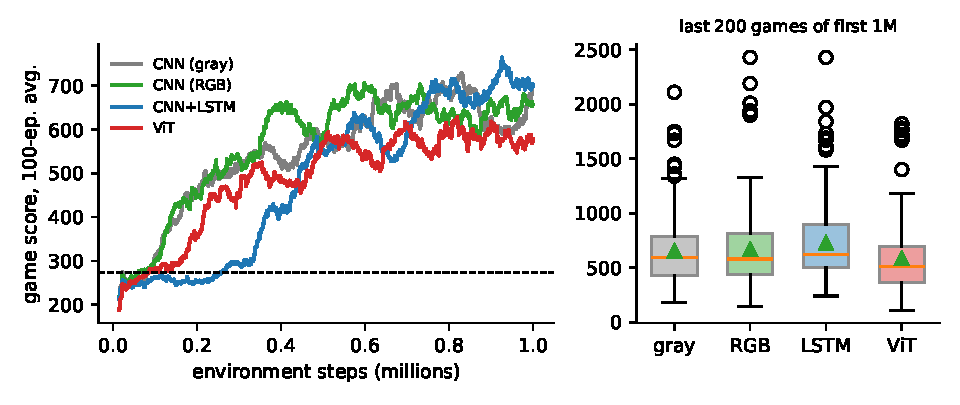
\includegraphics[width=0.78\linewidth]{figures/fig_first1M.pdf}
\caption{First 1 M steps. Left: 100-game moving average of the training score, dashed line is random play. Right: distribution of the last 200 games (triangle: mean). RGB $\approx$ gray; the LSTM is slightly ahead and the ViT slightly behind at this budget.}
\label{fig:first1m}
\end{figure}
RGB equals gray within one standard error, and the LSTM's lead (+70) is about two standard errors with a single seed. None of these gaps are decisive at 1 M steps.

\paragraph{P3: long fine-tuning.} With a small step penalty (\spen$=0.05$) and a lower learning rate, both sequence-aware models continued to improve rather than plateau (Figure~\ref{fig:curves}). Table~\ref{tab:stages} gives the training score by stage and Table~\ref{tab:final} the final summary.
\begin{figure}[t]
\centering
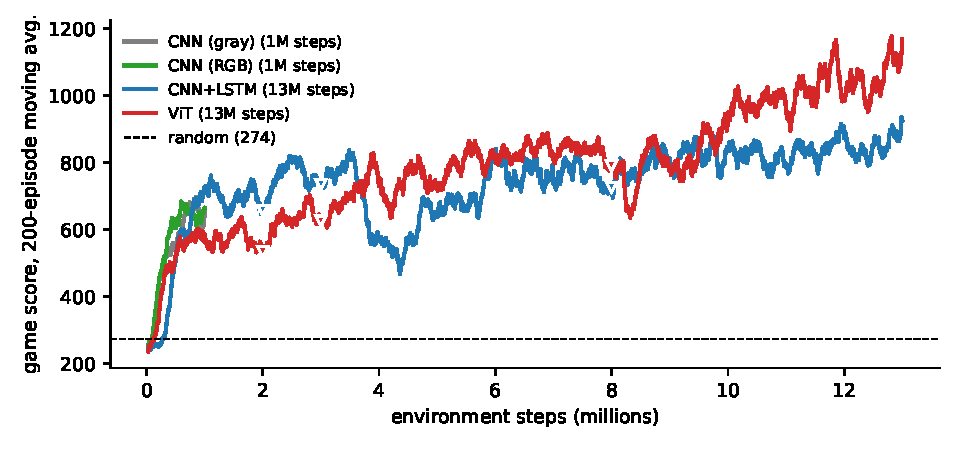
\includegraphics[width=0.88\linewidth]{figures/fig_learning_curves.pdf}
\caption{Training score (200-game moving average) for the best run of each model type. LSTM and ViT are chains of stages (triangles mark stage changes) of 2, 1, 5 and 5 M steps; after the first stage they use \spen$=0.05$ and a lower learning rate, so they are \emph{not} under the same conditions as the two 1 M-step CNNs.}
\label{fig:curves}
\end{figure}
\begin{table}[h]
\centering\small
\begin{tabular}{lcccc}
\toprule
Stage (cumulative steps) & pre (2 M) & P1 (3 M) & A (8 M) & C (13 M)\\
\midrule
ViT  & 492 & 655 & 818 & \textbf{1181}\\
CNN+LSTM & 665 & 729 & 744 & 967\\
\bottomrule
\end{tabular}
\caption{Training score (last 100 games of each stage). A branch that raised the death penalty to 10 for 1 M steps (stage B) scored 858 (ViT) and 732 (LSTM), i.e.\ no better than stage A.}
\label{tab:stages}
\end{table}
\begin{table}[h]
\centering\small
\begin{tabular}{lcccccc}
\toprule
Model & Steps & Mean & Median & P90 & Best game & Entropy\\
\midrule
CNN (gray) & 1 M & 652 & 580 & 1140 & 2260 & 1.75\\
CNN (RGB)  & 1 M & 640 & 560 & 1070 & 2460 & 1.77\\
CNN+LSTM   & 13 M & 900 & 800 & 1391 & 4600 & 1.54\\
ViT        & 13 M & \textbf{1125} & \textbf{975} & \textbf{1940} & 4720 & 1.76\\
\bottomrule
\end{tabular}
\caption{Last 300 training games of each model's best run (standard error of the mean: 19, 19, 25, 34). The score distribution is heavy-tailed, so the mean exceeds the median in all rows.}
\label{tab:final}
\end{table}
Re-scoring the ViT checkpoints during the last stage gave evaluation scores of 1115, 1208, 1296 and 1092 (20 games each, std 450--560, medians 905--1175), consistent with the training score of $\approx$1100--1180.

\paragraph{P4: RGB from gray and penalty magnitude.} Table~\ref{tab:sp} shows RGB networks initialised from a trained gray CNN (1 M steps) and trained with a ramping death penalty (2.5$\to$5$\to$10) under different step-penalty values. Only the setting with \spen$=2$ failed outright; its value loss was two orders of magnitude larger than in the other runs.
\begin{table}[h]
\centering\small
\begin{tabular}{lccccc}
\toprule
\spen & Steps trained & Train score (first 100 / last 100 games) & Eval (20 games) & Value loss (start$\to$end)\\
\midrule
0.05 & 10.0 M & 664 / 646 & $640\pm73$ & 1.3 $\to$ 1.7\\
0.3  & 24.0 M & 604 / 779 & $626\pm72$ & 3.5 $\to$ 2.8\\
0.5  & 3.0 M (stopped early) & 681 / 387 & -- & 15.3 $\to$ 13.7\\
2    & 7.65 M & 543 / 492 & $510\pm68$ & 394 $\to$ 283\\
\bottomrule
\end{tabular}
\caption{RGB-from-gray runs (one seed each). Eval is mean$\pm$standard error. The gray source model scores 608 and 828 in two separate 20-game evaluations (see \S\ref{sec:analysis}).}
\label{tab:sp}
\end{table}

\section{Analysis}
\label{sec:analysis}
\paragraph{What did the ViT learn?} The headline score gain is visible in behavioural counters rather than in survival alone (Figure~\ref{fig:behaviour}). Up to 8 M steps both ViT and LSTM sit at $\approx$0.6 ghosts and $\approx$1.0 pellets per game, the same level as the plateaued CNN. After 8 M steps the ViT rises to $\approx$1.06 ghosts and $\approx$1.58 pellets per game (last 1 M steps), while the LSTM stays at 0.60 and 0.92, and the ViT also survives about 10\% longer (from $\approx$650 to $\approx$740 steps/game). Because ghosts are worth 200--1600 points, doubling ghost captures explains most of the score increase. This partly overturns our earlier reading that no model had learned to hunt ghosts, but it appears only after $\sim$10 M steps, and our ghost counter cannot separate fruit from ghosts (see \S\ref{sec:experiments}).
\begin{figure}[t]
\centering
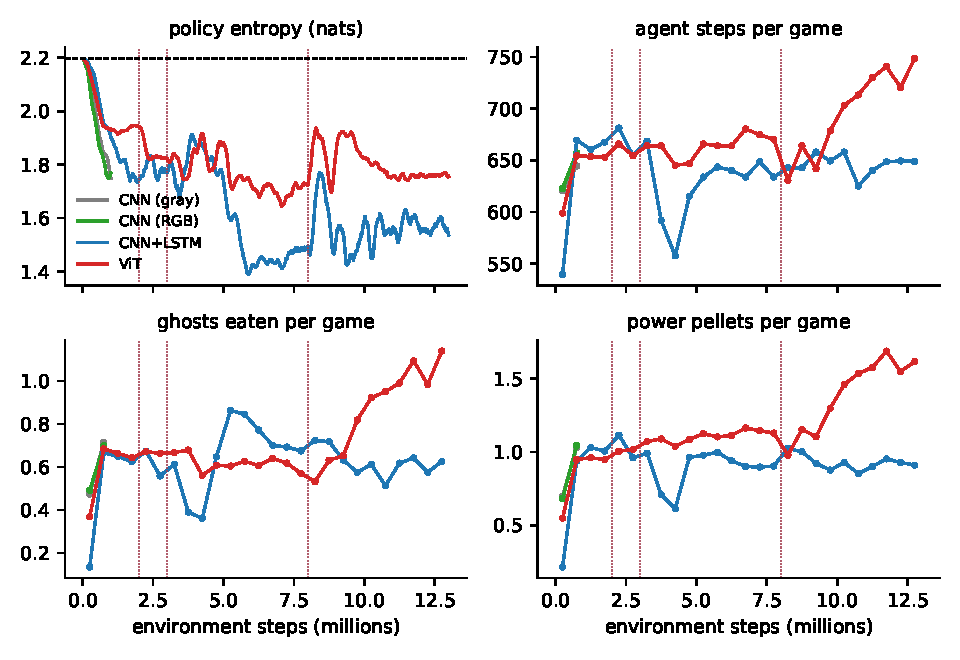
\includegraphics[width=0.88\linewidth]{figures/fig_behaviour.pdf}
\caption{Behaviour metrics in 0.5 M-step bins for the four best runs (dotted lines: stage changes). The ViT's gain after $\sim$8 M steps comes with more ghosts and pellets per game; the LSTM keeps lower policy entropy but gains little.}
\label{fig:behaviour}
\end{figure}

\paragraph{Penalty magnitude, value loss and collapse.} Penalties that are too large destroyed learning in two independent places. First, the RGB run with \spen$=2$: per-step cost $2$ over a typical $\approx$215-step life gives $\approx -430$ per life, far more than any positive reward in Eq.~\eqref{eq:reward} (a dot is 0.69). Value loss was $\approx$300--400 versus $\approx$1 elsewhere, and a continuation run degraded to near-random play (steps/life $\approx$128, almost no pellets). Second, when the best ViT was trained further with \dpen$=5$ and \spen$=0.3\to1\to0.5$ (shaded region of Figure~\ref{fig:collapse}), the training score fell from $\approx$1140 to $\approx$490 within one stage, and evaluation fell from 1092 to 434. Our explanation, which we have not isolated with a counterfactual run, is that with a negative per-step reward and termination on death, ending the life early becomes rational whenever \dpen{} is smaller than the penalty the agent expects to pay over the rest of the life ($\approx\spen\times 200$ steps). At \spen$=1$ that is $\approx$200, versus \dpen$=5$. This is consistent with the shorter lives (188--192 steps vs.\ $\approx$215) and with fewer pellets per life in the logs. Raising \dpen{} alone to 10 (stage B) did not collapse learning but did not help either. A practical outcome: a value-loss jump by 10$\times$ or more over a run's baseline is a cheap early warning that reward scale is wrong, and in the cases above it appeared long before the score did.
\begin{figure}[t]
\centering
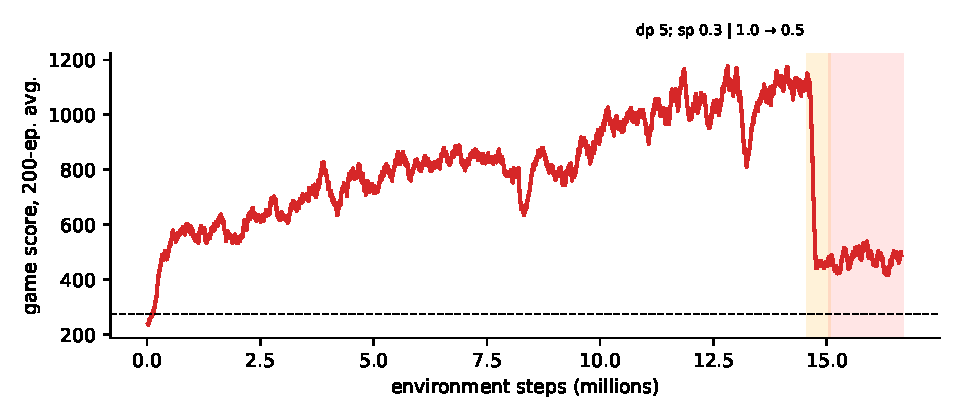
\includegraphics[width=0.82\linewidth]{figures/fig_vit_collapse.pdf}
\caption{ViT training score over the full 16.65 M-step chain. The shaded region marks the stages where we raised penalties (\dpen$=5$, \spen$=0.3$, then 1.0 and 0.5); the score drops from $\approx$1140 to $\approx$490 and does not recover.}
\label{fig:collapse}
\end{figure}

\paragraph{Does colour help? A single-frame check.} After eating a power pellet, a frame in RGB contained 116 blue pixels (frightened ghost). Its luminance in gray is 109, \emph{identical} to a common maze gray level (109), so the ghost is plausibly hard to distinguish in gray. Yet RGB did not improve the score or ghost captures: in the last 1 M steps both the gray and the RGB CNN eat 0.59 ghosts per game. We therefore cannot support H2 at this budget: the information may be recoverable from the gray image (e.g.\ via ghost motion), or the agent may not yet be able to exploit the signal. This is a single-frame analysis and we did not complete a direct behavioural test around frightened ghosts. A RAM-based ghost-state probe was written but not validated on Ms.\ Pac-Man, so we do not report it.

\paragraph{Evaluation noise limits what we can claim.} The same gray model scored 828 in one 20-game evaluation and 608 in another; a ViT checkpoint scored 748, 660 and 499 across three evaluations with the same seed set. With std 200--500 per 20 games, the standard error is 50--100, so any gap below $\sim$150 points between two models is not interpretable. We suspect unseeded action sampling and trajectory-dependent environment noise but did not identify the cause. For this reason Tables~\ref{tab:penalty}--\ref{tab:final} lean on thousands of training games, accepting their bias, and we describe single-seed comparisons as trends. This also tempers the architecture comparison: ViT vs.\ LSTM differ in learning rate, stage timing and seed count, so ``ViT $>$ LSTM'' is a hypothesis for future controlled testing, not a result.

\section{Conclusion}
\label{sec:conclusion}
Starting from a PPO agent stuck at $\sim$700 points, we tested reward shaping, RGB input and sequence models. The solid findings are: (1) long, low-learning-rate fine-tuning with a small step penalty let the ViT reach a training score of 1125 (best game 4720), with the main behavioural change being about twice as many ghosts eaten per game; (2) large penalties from the start (const-high) hurt, and penalties above a threshold ($\spen\ge0.3$ for the ViT, $\spen=2$ for the RGB CNN) cause collapse; (3) RGB input and a death-penalty curriculum gave no measurable benefit at 1--10 M steps; (4) evaluation noise of 100--200 points means many small gaps are not interpretable. The main limitations are one seed for most conditions, confounded changes between stages (learning rate, penalty, architecture), 20-game evaluations and a coarse ghost counter. We did not obtain DQN results on Ms.\ Pac-Man. Next steps are: run $\ge$3 seeds with $\ge$50 evaluation games and fixed action-sampling seeds; run a ViT/LSTM comparison under identical learning rate and step budget; repeat the 13 M-step schedule without the step penalty to separate its effect from training length; test exploration bonuses \citep{burda2019rnd}; and probe frightened-ghost behaviour directly.

\section*{Ethical Considerations}
\label{sec:ethics}
\textbf{Reward misspecification and what it teaches about deployment.} The clearest failure in this project was a reward-design error: a per-step penalty that made quitting early the best strategy, so the agent got \emph{worse} at the intended task while obeying the objective. The agent was only a game character, but the same mechanism (optimising a proxy that omits something important) matters when RL policies are used for resource allocation, content recommendation, or control. Our case is specific because the penalty was introduced to fix a visible symptom (idling), and the fix produced a harder-to-see failure; the problem was detected only by a diagnostic (value loss) that we happened to log. Mitigations: (i) log a small set of intended-behaviour metrics next to the shaped return (here: pellets, ghosts, steps per life) and stop training automatically when they diverge from the true objective, as we did with an early-stop threshold on training score; (ii) test every added penalty on a short run first, with value-loss and behaviour checks, before long training; and (iii) in a deployed setting, keep a human review step for any change to the reward function.

\textbf{Compute cost and misleading evidence.} Our results rest on 23 saved runs of up to 24 M steps each (about 84 M steps in total), run on a GPU laptop. Compute-hungry RL experiments carry an energy cost \citep{strubell2019energy}, and the cost is wasted when single-seed comparisons are mistaken for findings; over-confident claims can also lead other groups to repeat the same expensive experiments. Mitigations: report seeds, evaluation size and noise (as in \S\ref{sec:analysis}); release logs and the figure-generating script so others can reuse our runs; and prefer short multi-seed pilots before long runs.

\textbf{Game automation.} A pixel-only agent that plays a commercial game can, with modest changes, be used as a bot. For a 1980s arcade game the harm is low, but the same pipeline could be reused for online games, where automation breaks fair play. A mitigation is to share only the training code for the emulator environment, not any interface to live online services, and to state this intended scope in the repository's documentation.

\bibliographystyle{plainnat}
\bibliography{refs}

\appendix
\section{Hyperparameters and reproducibility}
\label{app:hparams}
\begin{table}[h]
\centering\small
\begin{tabular}{ll|ll}
\toprule
Parameter & Value & Parameter & Value\\
\midrule
Parallel envs $\times$ steps/rollout & $32\times512$ & Clip $\epsilon$ & 0.1\\
Epochs / minibatches & 4 / 4 & $c_1$ (value), $c_2$ (entropy) & 0.5, 0.01\\
$\gamma$, $\lambda$ & 0.99, 0.95 & Grad-norm clip & 0.5\\
Learning rate (from scratch) & $2.5\!\times\!10^{-4}$ & Fine-tuning learning rate & $10^{-4}$ or $5\!\times\!10^{-5}$\\
Frame skip, sticky prob. & 4, 0 & Max evaluation steps & 4500\\
ViT & patch 12, dim 128, depth 4, 4 heads & LSTM hidden & 512\\
\bottomrule
\end{tabular}
\caption{PPO and network hyperparameters. Hardware: RTX 3070 Ti Laptop GPU, PyTorch 2.3.1 (CUDA 12.1), Gymnasium 0.29.1.}
\end{table}
All figures and the numbers in the text are regenerated from the saved run logs by \texttt{Reports/paper/make\_figures.py}. Two evaluations of the same model can differ by 100--200 points (\S\ref{sec:analysis}), so re-running the 20-game evaluation will not reproduce the exact values in Table~\ref{tab:sp}.

\end{document}
